\chapter{Metodologia}
\label{c.metodologia}

Planeja-se dividir o estudo de acordo com as seguintes etapas:

\begin{itemize}
	\item[-] Levantamento bibliográfico
	\item[-] Análise e desenvolvimento das técnicas de detecção baseadas em assinatura utilizadas atualmente
	\item[-] Implementação Computacional
	\item[-] Análise dos resultados e conclusão da monografia.
\end{itemize}
A confecção da monografia vai ocorrer juntamente com o andamento das demais
etapas definidas durante toda a extensão do projeto. A ideia é utilizar
máquinas virtuais e emuladores para implementar em caráter de teste os
algoritmos de detecção baseados em assinatura sobre um conjunto de programas
contendo alguns programas já infectados com amostras de malware diversas para
observar, em termos gerais, a eficiência do tempo de execução dos algoritmos e
suas respectivas taxas de sucesso. O ambiente pode ser montado em qualquer
máquina que suporte a plataforma Windows e emulador Android, então não há
necessidade de que se reserve material da UNESP para uso exclusivo do projeto.
A figura a seguir ilustra o planejamento do projeto.
\begin{figure}[h]
\caption{\small Estrutura do projeto}
\centering
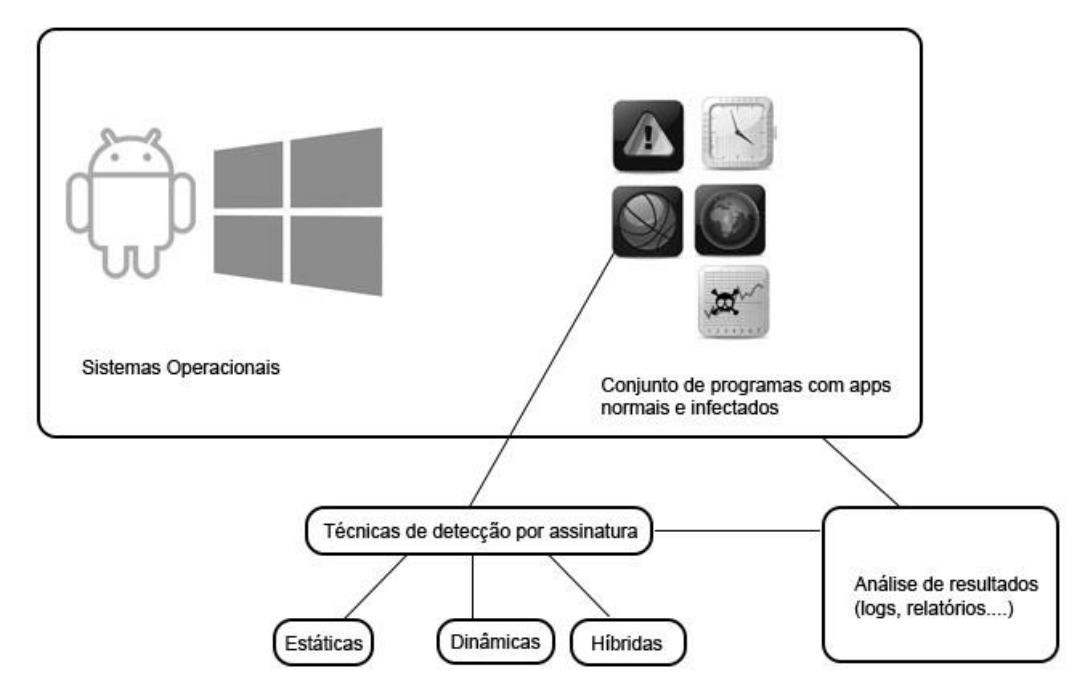
\includegraphics[scale=0.4]{figs/fig2}
\label{f.estrutura_projeto}
\legend{\small Fonte: Elaborada pelo autor.(2016)}
\end{figure}


